\section{System overview}
\label{sec:system_overview}

In this section, we provide a brief overview of the requests associated with this assignment, along with a description of the approach taken to fulfill them.
In the successive two sections instead, we describe in detail the control strategies implemented, and the analysis of the results obtained.

\subsection{Request}
\label{subsec:request}

For this assignment, we are asked to implement a feedback control strategy that is able to drive a \texttt{Turtlebot3} robot of the model \texttt{burger} through some predefined waypoints in the environment.

In particular, the waypoints are specified as a list of 3D coordinates in the world frame, where the first two coordinates represent the position of the vehicle in the plane, and the third coordinate represents the orientation of the vehicle in the world frame.

Also, along with this core request, we are asked to implement two control strategy such as:

\begin{itemize}
    \item A simple proportional controller, subjected to a set of constraint;
    \item A more advanced controller (no particular constraints on its choice).
\end{itemize}



\subsection{Waypoints}
\label{subsec:waypoints}

Before proceeding with the actual implementation of the control system, we show in Figure \ref{fig:waypoints} the waypoints used for this assignment.
These waypoints are provided along with the text of the assignment.

\begin{figure}[H]
    \centering
    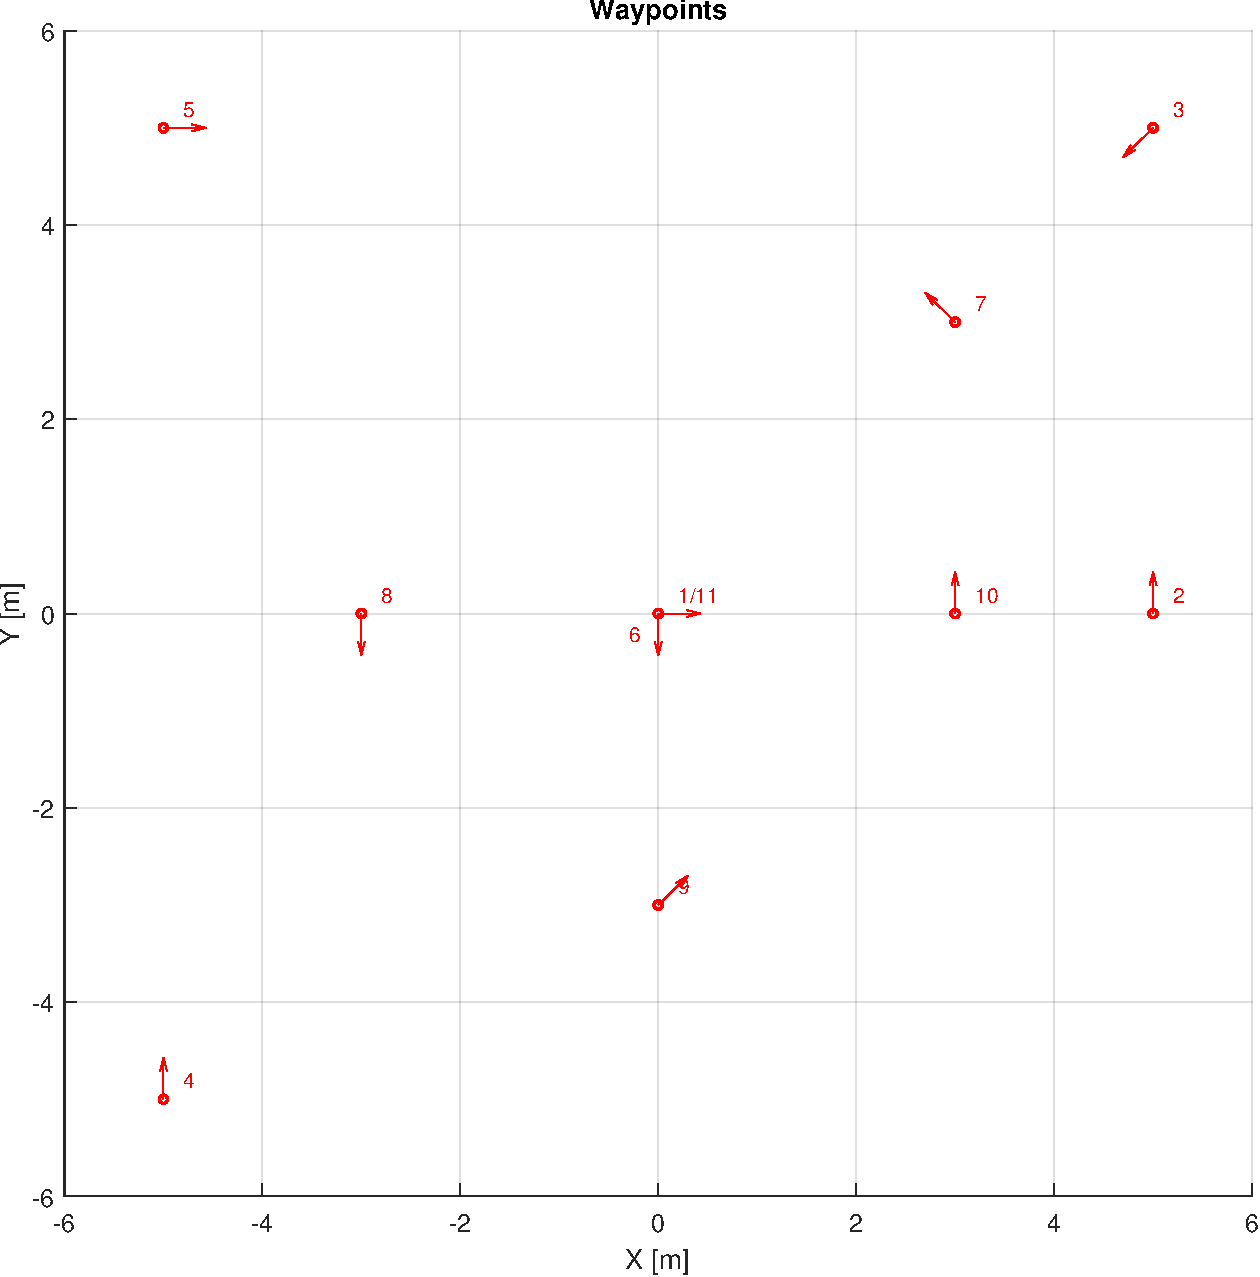
\includegraphics[width=0.6\textwidth]{./img/MATLAB/waypoints.pdf}
    \caption{Waypoints used for the simulation.}
    \label{fig:waypoints}
\end{figure}

In Figure \ref{fig:waypoints}, we can see the waypoints used for the simulation, which are represented as red dots in the world frame.
The arrow associated to each waypoint represents the orientation of the vehicle at that waypoint, which is given by the third coordinate of the waypoint list.



\subsection{Simulink model}
\label{subsec:simulink_model}

As already mentioned in the previous section, the logic of the feedback control loop is implemented in \texttt{Simulink}, which is a graphical programming environment for modeling, simulating and analyzing dynamic systems.
In Figure \ref{fig:simulink_model} we can see the Simulink model used for this assignment.

\begin{figure}[H]
    \centering
    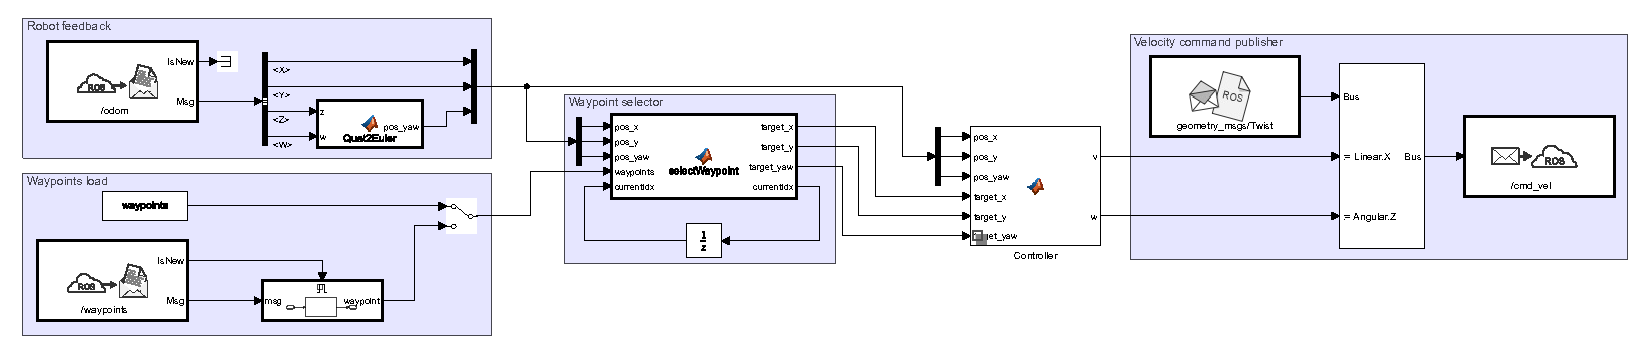
\includegraphics[width=1.0\textwidth]{./img/MATLAB/overview.pdf}
    \caption{Simulink model used for the implementation of the feedback control loop.}
    \label{fig:simulink_model}
\end{figure}

One can easily recognize the different components of the system thanks to the colored areas used to group the different blocks.
The main components of the system are:

\begin{itemize}
    \item Sensors readings: these blocks are used to subscribe to the \texttt{/odom} topic and to extract the data needed for the control system;
    \item Waypoint loader: this block is used to load the waypoints from either a workspace variable or a custom topic \texttt{/waypoints} on which the list of waypoints is published;
    \item Waypoint selector: this block is used to select the current waypoint from the list of waypoints, based on the current position of the vehicle and its history;
    \item Controller: this block is responsible for the logic of the feedback control loop. It computes the control commands to be sent to the vehicle based on the current position and orientation of the vehicle, and the current waypoint to be reached. The controller is implemented as a MATLAB function block, which allows for a more flexible implementation of the control logic. More details on the implementation of the controller are provided in the next sections;
    \item Command publisher: this block is used to publish the control commands to the \texttt{/cmd\_vel} topic, which is used by the vehicle to receive the control commands.
\end{itemize}

Notice that the commands sent to the vehicle are comprehensive of both linear and angular velocities.
In fact, a differential drive model is used internally by the robot to compute the wheel velocities based on the linear and angular velocities provided by the control system.

Inside the controller block, we can find the two different control strategies implemented for this assignment, namely a simple proportional controller and a more advanced controller based on Lyapunov analysis.
See Figure \ref{fig:controller_block} for an inside view of the controller block.

\begin{figure}[H]
    \centering
    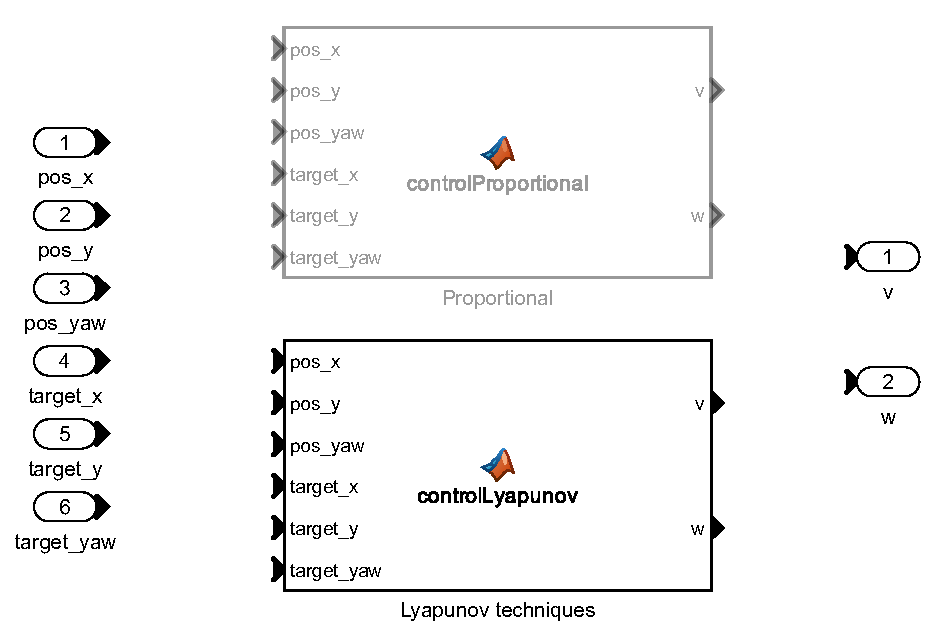
\includegraphics[width=0.9\textwidth]{./img/MATLAB/controller.pdf}
    \caption{Inside view of the controller block.}
    \label{fig:controller_block}
\end{figure}
